\documentclass[conference]{IEEEtran}
\IEEEoverridecommandlockouts
% The preceding line is only needed to identify funding in the first footnote. If that is unneeded, please comment it out.

 \usepackage{latexsym,amsmath,amssymb,amsfonts}
\usepackage[applemac]{inputenc}
\usepackage{rotating}
\usepackage{cite}
%\usepackage{graphicx}
\usepackage{epstopdf}
\usepackage{subfigure}
%\usepackage{color}
%\usepackage{xcolor}
%
%\usepackage{color}
\usepackage[dvipsnames]{xcolor}
%
\usepackage[normalem]{ulem}
\usepackage{isolatin1}
%\usepackage{caption}
%\usepackage{array,multirow,makecell}
%\usepackage{placeins}
%\usepackage{stackengine}
%\usepackage{hyperref}
\usepackage{fancybox}
\usepackage{colortbl}
\usepackage{float}
\usepackage{comment}
\usepackage{mathdots}
%\usepackage{lmodern}
%%%%%%%%%%%%%%%%%%%%%%%%%%%%%%%%%%%%%%%%%%%%%%%%%%%%%%%%%
\usepackage{dblfloatfix}
\usepackage{kantlipsum}
\usepackage{dblfloatfix}    % To enable figures at the bottom of page
\usepackage{graphicx} % [demo] option for empty figure
\usepackage{placeins}
\usepackage{marginnote}
\usepackage{url}
\usepackage{bm}
\usepackage[ruled,vlined]{algorithm2e}
%\usepackage{algorithm}
\usepackage{algorithmicx}
\usepackage{algpseudocode}
%%%%%%%%%%%%%%%%%%%%%%%%%%%%%%%
%%%
\newtheorem{prb}{\it Problem}%[section]
\newtheorem{theorem}{\it Theorem}%[section]
\newtheorem{lemma}{\it Lemma}%[section]
\newtheorem{definition}{\it Definition}
\newtheorem{remark}{\it Remark}%[section]
\newtheorem{assumption}{\it Assumption}%[section]
\newtheorem{example}{\it Example}%[section]b
\newtheorem{annex}{\it Annexe}%[section]b
\newtheorem{prop}{\it Proposition}%[section]b








\def\BibTeX{{\rm B\kern-.05em{\sc i\kern-.025em b}\kern-.08em
    T\kern-.1667em\lower.7ex\hbox{E}\kern-.125emX}}
\begin{document}

\title{Detection and Isolation of False Data Injection Attack via Unknown Input Observer *\\
{\footnotesize \textsuperscript{*}Note: Sub-titles are not captured in Xplore and
should not be used}
\thanks{Identify applicable funding agency here. If none, delete this.}
}

\author{\IEEEauthorblockN{1\textsuperscript{st} ....}
\IEEEauthorblockA{\textit{dept. name of organization (of Aff.)} \\
\textit{name of organization (of Aff.)}\\
City, Country \\
email address or ORCID}
\and
\IEEEauthorblockN{2\textsuperscript{nd} ....}
\IEEEauthorblockA{\textit{dept. name of organization (of Aff.)} \\
\textit{name of organization (of Aff.)}\\
City, Country \\
email address or ORCID}
\and
\IEEEauthorblockN{3\textsuperscript{rd} Given Name Surname}
\IEEEauthorblockA{\textit{dept. name of organization (of Aff.)} \\
\textit{name of organization (of Aff.)}\\
City, Country \\
email address or ORCID}
}

\maketitle

\begin{abstract}
The estimation and detection of cyber-attacks in connected and autonomous vehicles(CAV) are critical for ensuring security and increasing vehicle automation level. This paper presents a solution to estimate cyber-attacks in cooperative adaptive cruise controllers (CACC) following a vehicle with a preceding vehicle. A new method is proposed where the output of the original is shifted to obtain a new system satisfying the so-called observer matching condition(OMC). Furthermore, the dynamic is represented in descriptor system form and a strong delayed observer is designed to achieve an asymptotic estimation of both the cyber-attack and and state of the CACC system. Moreover, by the mean of Lyapunov stability theory, sufficient conditions are proposed, expressed in terms of Linear Matrix Inequality, to design the linear unknown input observer(UIO). Several test scenarios are applied to show the effectiveness of the proposed algorithm.
\end{abstract}

\begin{Keywords}
Keywords: Unknown input observers, Observer matching condition, strong detectability, Lyapunov stability, Intelligent vehicles,cyber-attack.
\end{Keywords}

\section{Introduction}

%Connected Autonomous Vehicles and CACC:\\
Connected autonomous vehicles (CAVs) have transformed traditional transportation systems by enabling wireless communication and interaction among vehicles. A notable advancement in this domain is Cooperative Adaptive Cruise Control (CACC), which extends the functionality of Adaptive Cruise Control (ACC). ACC automates vehicle speed adjustments based on preceding traffic, while CACC enhances this by incorporating inter-vehicle communication. Through this communication, vehicles can form platoons, maintaining consistent distances and potentially improving traffic flow.

%Cyber-Attack Detection in Vehicular Systems:\\
The integration of wireless communication and data exchange in CAVs brings forth concerns regarding cyber-attacks. Cyber-attack detection is crucial to ensure the integrity, safety, and reliability of vehicular communication systems. Attacks can manifest as false data injection, Denial of Service (DoS), eavesdropping, or interference, targeting communication channels or sensor systems. Detecting and mitigating these attacks are essential to maintaining the proper functioning of CAVs and ensuring road safety.

%(Talk about method in the literature )  PI-Observer , Sliding mode observer , Set-Membership

%Unknown Inputs in CACC: 
In the realm of CACC, the presence of unknown inputs adds complexity to the control system. Unknown inputs can arise from various sources, including sensor faults, cyber-attacks, and disturbances. Detecting and estimating these unknown inputs is essential for maintaining the stability and safety of the control system. Traditional methods, such as Unknown Input Observers (UIOs), are employed to estimate these inputs and mitigate their adverse effects on the system.






\section{Problem Formulation}

\begin{figure}[htp]
    \centering
    \includegraphics[width=8cm]{img/illutration_cacc.png}
    \caption{Illustration of CACC working on a vehicle platoon}
    \label{fig_pre_fol}
\end{figure}



\subsection{Collaborative Adaptive Cruise Control Model}
The dynamics of vehicle $i^{th}$ are Position-Velocity-Acceleration third-order linear model given by
\begin{equation}\label{eq_1}
      \left\{ \begin{array}{l}
        \dot{p}_i(t) =v_i(t) \\
        \dot{v}_i(t)  =a_i(t) \\
        \dot{a}_i(t)  =\frac{1}{\tau_i} u_i(t)-\frac{1}{\tau_i} a_i(t)\end{array}\right.
\end{equation}  
where
\begin{itemize}
\item $p_i(t), v_i(t)$ and $a_i(t)$ denote the position, velocity and
acceleration of the $i^{th}$  vehicle, respectively;
\item $u_i(t)$ is the $i^{th}$ vehicle's control input representing the desired
driving/braking force or acceleration;
 \item $\tau$ is the engine constant time lag. 
 \end{itemize}
 
The system \eqref{eq_1} can be rewritten as follows:
\begin{equation}\dot{x}_{i}(t)=\left[\begin{array}{c c c}{{0}}&{{1}}&{{0}}\\ {{0}}&{{0}}&{{1}}\\ {{0}}&{{0}}&{{-\tau^{-1}}}\end{array}\right]x_{0}(t)+\left[\begin{array}{c}{{0}}\\ {{0}}\\ {{\tau^{-1}}}\end{array}\right]u_{r}(t).\end{equation}


% The output yi of vehicle i is given by\\

% $y_{i}(t)=C x_{i}(t)=\left[{\begin{array}{r r r}{1}&{0}&{0}\\ {0}&{1}&{0}\end{array}}\right]x_{i}(t).$
% In this study, the control strategy is similar to the one that
% is presented [bla] 

% were x = [x1, v1, a1] > R2n are the states of all the vehicles in the platoon, A 2 R2n ⇥ 2n, B 2
% R2n⇥2, C 2 R2n⇥2n,

% The desired spacing between vehicles in the constant time-gap spacing policy is not constant but is linear function of speed:
% \begin{equation}
%     Desired\;Spacing=L_{i}+h\dot{x}_{i}
% \end{equation}

 To maintain a constant distance between two consecutive following vehicles, we use a constant time-gap spacing policy. Therefore, the spacing error can be written as: 
\begin{equation} \label{spacing_e}
 \overline{{{\varepsilon}}}_{i}=\varepsilon_{i}+h{v}_{i}=x_{i}-x_{i-1}+L_{i}+h{v}_{i},
\end{equation}
where ${L_i}$ is a constant and $h$ is the time-gap.
Based on~\eqref{spacing_e}, the controller is given by :
\begin{align}\label{controller}
        u_{\text{syn}}&=-k_{1}{a}_{i-1}+(k_{1}+h k_{1}k_{2}){a}_{i}-\frac{1}{h}(1-h k_{1}k_{2})\dot{\varepsilon}_{i}\notag\\
        &~~-\frac{k_{2}}{h}\varepsilon_{i}-k_{2}\dot{x}_{i},
\end{align}
where ${a}_{i-1}$ is the acceleration of the preceding vehicle obtained by using inter-vehicle communication.
The variables $k_1$ and $k_2$ are controller design parameters. In \cite{..}, if the gain $k_1$ is chosen so as to satisfy $-k_{1}h >\tau$, then the ACC controller \eqref{controller} is string 
stable, no matter how small the value of the time gap $h$. 

\subsection{CACC model under cyber-attack model}
In CACC platoons, the acceleration sent via V2V communication is not always reliable because it can be tampered with by an attacker. The transmitted signal $a_{c}$ while considering cyber-attacks can be represented as
$a_{c}={a}_{i-1}+f_{c}$.

%\begin{remark}
%{\color{red}{je ne comprend pas la phrase ???????}
    Some typical attacks can be understood as a false signal added to the transmission :  
message falsification attacks and replay attacks, DOS. For example the case of DOS , by using Taylor's series expansion, the delayed signal $a_{i-1}(t-\tau_d )$ can be written as
\begin{equation}\mu(t-\tau_d ) = a_{i-1}(t) -\dot{a}_{i-1}(t)\tau+ \text{H.O.T}\end{equation}
So the delay can simply be presented as :
\begin{equation}\mu(t-\tau_d ) = a_{i-1}(t) + f_d. \end{equation}
% About why send acceleration rather than send control input $u$, from many papers. Maybe acceleration is more versatile, because, in case of a non-homogenous platoon, the control input is not the same. 
%}
%\end{remark}

Under a cyber-attack, the following vehicle receives $\mu$, and 
will utilize the transmitted signal in its controller \eqref{controller}: 

% \begin{align} \label{control_uc}
%         u_{s y n}&=\left(h k_1 k_2\right) \mu-\left(k_1+h k_1 k_2\right) f_c-k_2 \dot{x}_i  \notag\\
%        & +\frac{k_2}{h} \delta_i-\left(k_1+h k_1 k_2\right) \ddot{\delta}_i\notag\\
%        &+\frac{1}{h}\left(1-h k_1 k_2\right) \dot{\delta}_i -\frac{k_2}{h}\left(L_i-l_{i-1}\right)
%     \end{align}
\begin{align}\label{control_uc}
        u_{\text{syn}}&=-k_{1}\mu+(k_{1}+h k_{1}k_{2}){a}_{i}-\frac{1}{h}(1-h k_{1}k_{2})\dot{\varepsilon}_{i}\notag\\
        &~~-\frac{k_{2}}{h}\varepsilon_{i}-k_{2}\dot{x}_{i},
\end{align}

% $\begin{array}{c}{{u_{s y n}=-k_{1}a_{c}+(k_{1}+h k_{1}k_{2})\ddot{x}_{i}-{\frac{1}{h}}(1-h k_{1}k_{2})\dot{\varepsilon}_{i}}}\\ {{-{\frac{k_{2}}{h}}\varepsilon_{i}-k_{2}\dot{x}_{i}}}\end{array}$

As shown in Fig.~\ref{fig_pre_fol}, the radar-measured rear-to-bumper distance from the following vehicle to the preceding vehicle, this distance can be defined as
\begin{equation} \label{distance_error}
    \delta_{i}=p_{i-1}-p_{i}-l_{i-1},
\end{equation}
where $l_{i_1}$ is the length of the preceding vehicle. Then, we have 
\begin{equation} \label{error_state}
    \begin{aligned}
        & \dot{\delta}_i={v}_{i-1}-{v}_i \\
        & \ddot{\delta}_i={a}_{i-1}-{a}_i \\
        & \dddot{\delta_{i}}=\dot{a}_{i-1}-\dot{a}_i
    \end{aligned}
\end{equation}


where $\dot{\delta}_{i}$, $\ddot{\delta}_{i}$, and $\dddot{\delta}_{i}$ are the relative speed, acceleration, and jerk (rate of acceleration changes) between the preceding and following vehicle. By using \eqref{distance_error} and \eqref{error_state}, the controller \eqref{control_uc} becomes 
\begin{align}\label{control_new}
        u_{s y n}&=\left(h k_1 k_2\right) a_c-\left(k_1+h k_1 k_2\right) f_c-k_2 \dot{x}_i \notag\\
       &~~ -\left(k_1+h k_1 k_2\right) \ddot{\delta}_i+\frac{1}{h}\left(1-h k_1 k_2\right) \dot{\delta}_i+\frac{k_2}{h} \delta_i \notag\\
       & ~~-\frac{k_2}{h}\left(L_i-l_{i-1}\right)
\end{align}
We directly obtain the acceleration information of the preceding 
vehicle using wireless communication. Thus, without considering its lower-order dynamics, the jerk of the preceding vehicle is assumed to be zero:
\begin{equation}\label{jerk0}
    \dot{a}_{i-1} = 0    
\end{equation}
Substituting equation~\eqref{control_new} into \eqref{eq_1} and using \eqref{jerk0}, we obtain 
\begin{align}
    \ddot{\delta}_{i}&=\frac{1}{\tau}\Big\{(1-h k_{1}k_{2})\mu-(1-k_{1}-h k_{1}k_{2})f_{c}+k_{2}\dot{x}_{i}\notag\\
    &+(k_{1}-1+h k_{1}k_{2})\delta_{i}\notag\\ 
    &-\frac{k_{2}}{h}(1-h k_{1}k_{2})\delta_{i}-\frac{k_{2}}{h}\delta_{i}
    \end{align}
Finally, the interaction between two cars in a CACC scenario can be modeled, from the perspective of the following car $i$, as:
\begin{equation}\label{CACC}
      \left\{ \begin{array}{l}
        \dot{x}=A x+B \dot{x}_i+F \mu+\Delta-W f_c \\
         y = Cx,\end{array}\right.
\end{equation}  
where 
\begin{equation}
    \begin{aligned}
        A & =\left[\begin{array}{ccc}
        0 & 1 & 0 \\
        0 & 0 & 1 \\
        -k_2 / \tau h & -k_3 / \tau h & \left(k_1-k_3\right) / \tau
        \end{array}\right], \\
        B & =\left[\begin{array}{c}
        0 \\
        0 \\
        k_2 / \tau
        \end{array}\right], \quad F=\left[\begin{array}{c}
        0 \\
        0 \\
        k_3 / \tau
        \end{array}\right], \Delta=\left[\begin{array}{c}
        0 \\
        0 \\
        k_2\left(L_i-l_{i-1}\right) / \tau h
        \end{array}\right] \\
        W & =\left[\begin{array}{c}
        0 \\
        0 \\
        \left(k_3-k_1\right) / \tau
        \end{array}\right], \quad C=\left[\begin{array}{lll}
        1 & 0 & 0 \\
        0 & 1 & 0
        \end{array}\right].
    \end{aligned}
\end{equation}


\section{Proposed Mechanism}
\label{sec2}
As we have discussed previously, the CACC can be vulnerable to cyber-attacks that are most of the time unknown. From a dynamic system perspective, this is considered as an unknown input. We therefore introduce an unknown input observer (UIO) to detect attacks and maintain vehicles stability. 

\subsection{Model and Assumptions}
To implement the attack detection and defense mechanism, we discretize the dynamics model~\eqref{CACC}: 
\begin{equation}\label{CACC_discretized}
      \left\{ \begin{array}{l}
        x_{k+1} = A_{d}x_{k}+B_{d}u_{k}+F_{d}\mu_{k}-W_{d}f_{c\,k}+\Delta_{d}\\ 
        y_{k} = C_{d}x_{k}
   \end{array}\right.
\end{equation}  
with $A_{d}=(I_{3}+T_{s}A),\,B_{d}=\,T_{s}B,\,F_{d}=T_{s}F,\,W_{d}=T_{s}W,\,\Delta_{d}=T_{s}\Delta,\,C_{d}=T_{s}C,$, and $T_s$ being the sampling time.

\begin{assumption}
The necessary and sufficient conditions for the system in ~\eqref{CACC_discretized} to have an UIO are:
\begin{enumerate}
    \item rank($CE$)=rank($E$)
    \item $(C,G)$ is detectable.
\end{enumerate}

\end{assumption}

We can easily check the first condition
Unfortunately, The second condition concerns the satisfaction of {\color{red}$rank = rank()$}. This condition is very important in the sense that it allows to inverse of the matrix $CW$ to reconstruct the unknown input. It is commonly known as the Observer Matching Condition (OMC).
We begin by representing From 10, we write:

We have rank($CW$) $\neq$ rank($W$), and we conclude that the observer cannot exist for the system {\color{red}(3.1)}.
To overcome the rank condition that is not satisfied, it is necessary to do {\color{red}bla bla .}
$y_{k}=C_{d}(A_{d}x_{k-1}+B_{d}u_{k-1}+F_{d}\mu_{k-1}-W_{d}f_{c\,k-1}+\Delta_{d}),$
we can easily verify that: $$C_{d}B_{d}=C_{d}F_{d}=C_{d}W_{d}=C_{d}\Delta_{d}=0$$
hence $y_{k}=C_{d}A_{d}x_{k-1}.$
If we consider the change of variables:
\begin{equation}
    \begin{aligned}
        {Z_{k+1}} &=A_{d}z_{k}+B_{d}\bar{u}_{k}+F_{d}\bar{\mu}_{k}-W_{d}v_{k}+\Delta_{d}\\ 
        y_{k} &=\bar{C}_{d}z_{k}
    \end{aligned}
\end{equation}
where ${\cal Z}_{k}=x_{k-1},\;\bar{u}_{k}=u_{k-1}\;,\bar{u}_{k}=\mu_{k-1},\;v_{k}=fc_{k-1}\ and$ $\bar{C_d} = C_{d}A_{d}$
now we will verify the UIO existence condition namely OMC as follows: 
\begin{equation}
    \bar{C}_{d}W_{d}=\left[\begin{array}{c c c}
    0 \\
    0 \\
    {{T_{s}^{3}(k_{3}-k_{1})}}
    \end{array}\right]
\end{equation}
Therefore, $rank(\bar{C}_{d}W_{d})=rank(W_{d})$ when $T_s \doteq 0 $ . Finally, we conclude that there exists an unknown input observer for the system {\color{red}(3.6)} 
\subsection{Observer structure}
In order to deal with the unknown inputs due to the cyber-attack, $f_c$ will be considered as a state of the system. Using the new extended state vector, the original system is converted 
to the descriptor system form.The state vector that includes  $f_c$ is defined as : $\xi_{k}=[z_{k}^{r}\ v_{k}]^{r}$. We obtain the following discrete-time linear descriptor system:
% \begin{equation}
%     \left\{\begin{array}{r}
%     E\xi_{k+1}=A_{\xi}\xi_{k}+B_{\xi}\bar{u}_{k}+F_{\xi}\bar{u}_{k}+\Delta_{\xi}\\ 
%     {y_{k}=C_{\xi}\xi_{k}}
%     \end{array}\right.
% \end{equation}

\begin{equation}
    \left\{\begin{array}{c}
    E \xi_{k+1}=A_{\xi} \xi_k+B_{\xi} \bar{u}_k+F_{\xi} \bar{\mu}_k+\Delta_{\xi} \\
    y_k=C_{\xi} \xi_k
    \end{array}\right.
\end{equation}


Now let us consider the following observer structure to estimate states and unknown input simultaneously:
\begin{equation}
    \left\{\begin{array}{c}
        w_{k+1}=N w_{k}+L y_{k}+M\bar{u}_{k}+G\bar{\mu}_{k}+\ P_{z}\Delta_{\xi}\\ \hat{\xi}_{k}=w_{k}+Q_{z}y_{k}
    \end{array}\right.
\end{equation}


\begin{theorem}
    Assume there exist $P = P^\top > 0$, $\lambda > 0$,  $N, L, M, G, P_{z}$ and $Q_z$ such that:
\begin{equation}\label{LMI}
    S=\left[\begin{array}{c c c}{{A_{z}^{\ T}P A_{z}-A_{z}^{\ T}X C_{\xi}-C_{\xi}^{\ T}X^{T}A_{z}-P}&{{X C_{\xi}}}\\ {{\{X C_{\xi}}}}&{{-P}}\end{array}\right]<0
\end{equation}
%}
Then the estimation error $\tilde{x}(t)$ is exponentially stable.
\end{theorem}

\begin{proof}
    

 our goal is to design Observer matrices $N, L, M, G, P_{z}$ and $Q_z$ such that the estimation error ${\widetilde\xi}_{k}={\xi}_{k}-{\hat{\xi}}_{k}$ converges towards zero. We define the estimation error\\
${\widetilde\xi}_{k}={\xi}_{k}-{\hat{\xi}}_{k}={\xi}_{k}-w_{k}+Q_{z}C_{\xi}{\widetilde\xi}_{k}=\left(I_{4}-Q_{z}C_{\xi}\right){\widetilde\xi}_{k}-w_{k},$
We consider the following condition

\begin{equation}\label{CO_PEQC}
    P_{z}E+Q_{z}C_{\xi}=I_{n},
\end{equation}

thus, we obtain \\
\begin{equation}
    \widetilde\xi_{k}=P_{z}E\widetilde\xi_{k}-w_{k}
\end{equation}

using (\ref{CO_PEQC}), we obtain 
\begin{equation}\label{eQObs1}
 \widetilde{\xi}_{k+1}=N\widetilde\xi_{k}+(P_{z}A_{\xi}+N P_{z}E \\
 -L C_{\xi})\xi_{k}+(P_{z}B_{\xi}-M)\widetilde{u}_{k}+(P_{z}F_{\xi}-G)\widetilde{u}_{k}
\end{equation}

we can always choose $L$ such that
\begin{equation}\label{L}
    L = -K + NQ_z
\end{equation}

where K is a matrix of appropriate dimension. Substituting (\ref{L}) into the error equation (\ref{eQObs1}) we get
\begin{align*}
    \tilde{\xi}_{k+1}&=N \tilde{\xi}_k+\left(P_z A_{\xi}-N+K C_{\xi}\right) \xi_k\\
    &+\left(P_z B_{\xi}-M\right) \bar{u}_k+\left(P_z F_{\xi}-G\right) \bar{\mu}_k
\end{align*}


The observer (3.8) will estimate asymptotically  in other words tend to zero asymptotically, if the following conditions are satisfied\\

i) $N$ is a Hurwitz matrix, i.e., if $\lambda$ is the eigenvalue of $N$ then we have $\forall \lambda \in \mathbb{C},|\lambda|<1$.\\
ii) $N=P_z A_{\xi}-K C_{\xi}$.\\
iii) $P_z B_{\xi}=M$.\\
iv) $P_z F_{\xi}=G$.\\

% ${}[P_{z}\,Q_{z}]=\left[C_{\xi}\right]^{+}=\left[C_{\xi}\right]^{T}\left(\left[{E\atop C_{\xi}}\right]\left[C_{\xi}\right]^{T}\right)^{-1},$

we can compute $P_z$ and $Q_z$  using the following formula
\begin{equation}
    \left[\begin{array}{ll}
    P_z & Q_z
    \end{array}\right]=\left[\begin{array}{l}
    E \\
    C_{\xi}
    \end{array}\right]^{+}=\left[\begin{array}{c}
    E \\
    C_{\xi}
    \end{array}\right]^T\left(\left[\begin{array}{c}
    E \\
    C_{\xi}
    \end{array}\right]\left[\begin{array}{c}
    E \\
    C_{\xi}
    \end{array}\right]^T\right)^{-1}
\end{equation}

If all the above conditions are satisfied, the error dynamic is given by :

\begin{equation}
    \widetilde\xi_{k+1}=N\widetilde\xi_{k}
\end{equation}

Let us consider the discrete-time candidate Lyapunov function 
\begin{equation}
    V_{k}=\bar{\xi}_{k}^{\ T}P\bar{\xi}_{k}
\end{equation}

%we will obtain : 
%\begin{equation}
%    \Delta V_{k} < 0
%\end{equation}

The objective is to find $K$ and $P$ such that the following quantity is negative
\begin{equation}
    (P_{z}A_{\xi}-K C_{\xi})^{T}P(P_{z}A_{\xi}-K C_{\xi})-P < 0
\end{equation}

By applying Schur complement we obtain the following LMI
\begin{equation}\label{LMI}
    S=\left[\begin{array}{c c c}{{A_{z}^{\ T}P A_{z}-A_{z}^{\ T}X C_{\xi}-C_{\xi}^{\ T}X^{T}A_{z}-P}&{{X C_{\xi}}}\\ {{\{X C_{\xi}}}}&{{-P}}\end{array}\right]
\end{equation}
\end{proof}



\begin{figure}[htp]
    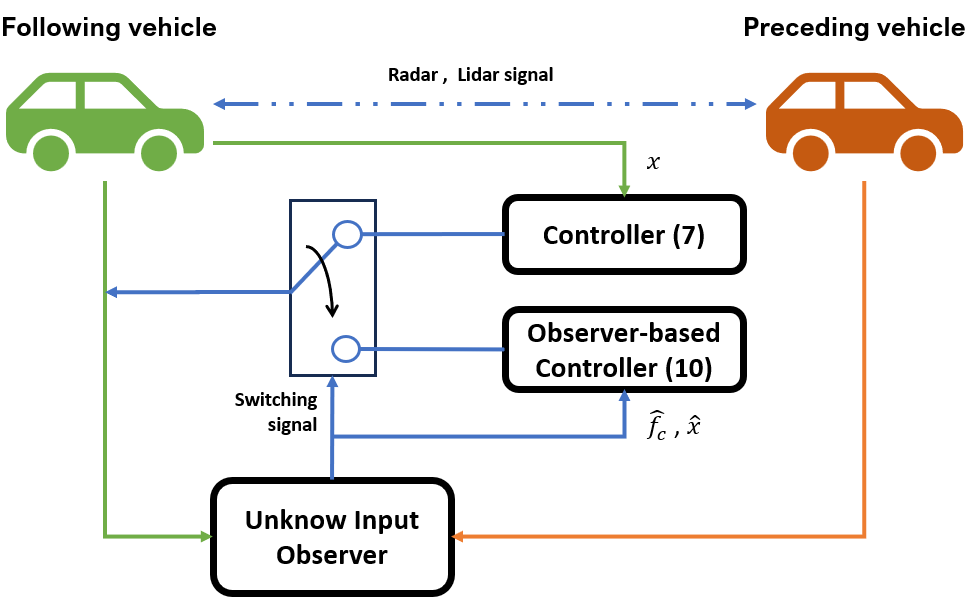
\includegraphics[width=9cm]{img/control_obser.png}
    \caption{UIO state estimation under constant attack}
    \label{fig:obser_control}
\end{figure}













\section{Simulation results}
We will explore two simulation scenarios, outlined below: 
\begin{description}
    \item[\textbf{Case 1:}]~~Constant attack signal
\begin{equation}
    f_c(t)=\left\{\begin{array}{lc}
    3(t-10) & t\geq10 \\
    0 & otherwise 
    \end{array}\right.
\end{equation}

%\begin{figure}[htp]
%    \centering
%    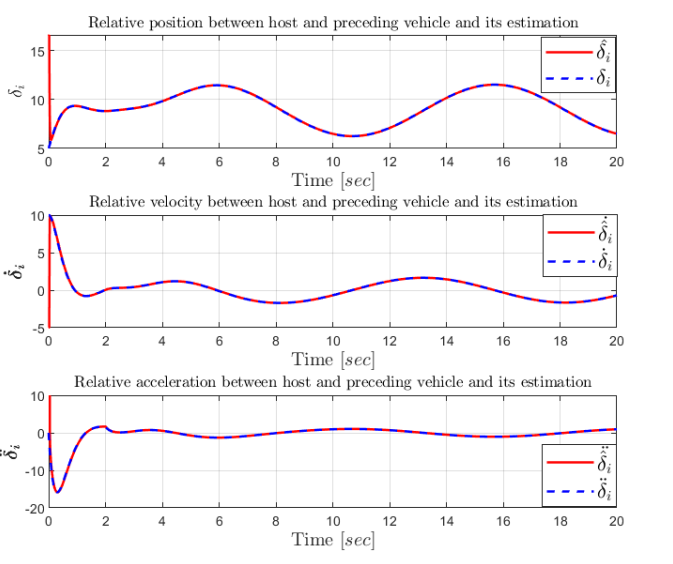
\includegraphics[width=8cm]{img/state_est.png}
%    \caption{UIO state estimation under constant attack}
%    \label{fig:galaxy}
%\end{figure}
\item[\textbf{Case 2 :}]~~~Time-varying attack signal
\begin{equation}
    f_c(t)=\left\{\begin{array}{lc}
    0 & 0<t<4 \\
    10 \sin (5 \pi t) \exp(-0.01 . t) & 4 \leq t<8 \\
    \exp(-0.02 \sin (5 \pi t) t) & 9 \leq t<16 \\
    0 & 16 \leq t<20
    \end{array}\right.
\end{equation}
\end{description}





\begin{table}
\centering
\begin{tabular}{|c|c|c|}
\hline
Parameter  & Value  & Unit  \\
\hline
$\tau$ & 0.4 & Row 1, Column 3 \\
$L_{i}$ & 7.3 & Row 2, Column 3 \\
$l_{i}$ & 5 & Row 2, Column 3 \\
$h$ & 0.5 & Row 2, Column 3 \\

\hline
\end{tabular}
\caption{Autonomous vehicles system parameters}
\label{tab:simple}
\end{table}

We solve (\ref{LMI}) for the observer gain using YALMIP. The observer gain is found to be eual 

$K = \left[\begin{array}{l l l}{{0.250{2}}}&{{}}&{{-0.005}}\\ {{-0.0018}}&{{}}&{{1.0000}}\\ {{0.2189}}&{{}}&{{-99.9950}}\\ {{-9.6978}}&{{}}&{{2757.1}}\end{array}\right]$

State estimation: From the fig, we see that the observer is able to produce a good estimation of 
the position, velocity, and acceleration. We perceive as well the effect of unknown input 
compensation, the ripples in velocity and acceleration from 4 to 8sec

Unknown input reconstruction and transmitted acceleration: In both cases (constant and 
time-varying) fault, the observer succeeded in reconstructing the attack. However, after two samples 
the observer design was based on the linear descriptor system (3.7) which is a two 
samples-delayed version of the system (3.5). The figure shows the difference between real and 
faulty transmitted acceleration, even when the signal is false, the SA-ACC control system is  immune against and this is thanks to the observer.
One problem with the observer is the transient phase of the cyber-attack estimation. This 
undesired phenomenon can be reduced either by reducing the observer gain (increase 
robustness) or adding a saturation

\begin{figure}[htp]
    \centering
    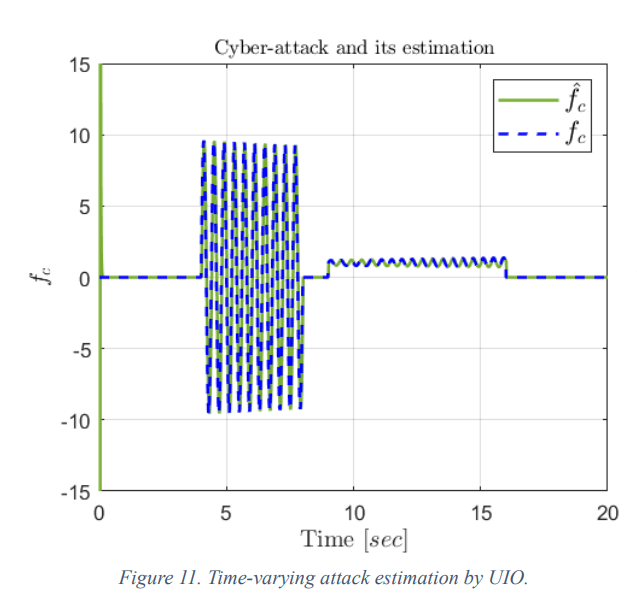
\includegraphics[width=8cm]{img/cyber_atk_est.png}
    \caption{UIO state estimation under constant attack}
    \label{fig:galaxy}
\end{figure}

\section{Experimental Results}
The first robot receives the excitation signals from a computer through wireless
connection, where the second and third robots are connected to the first and second robots, respectively, via a V2V
communication network.
\begin{figure}[htp]
    \centering
    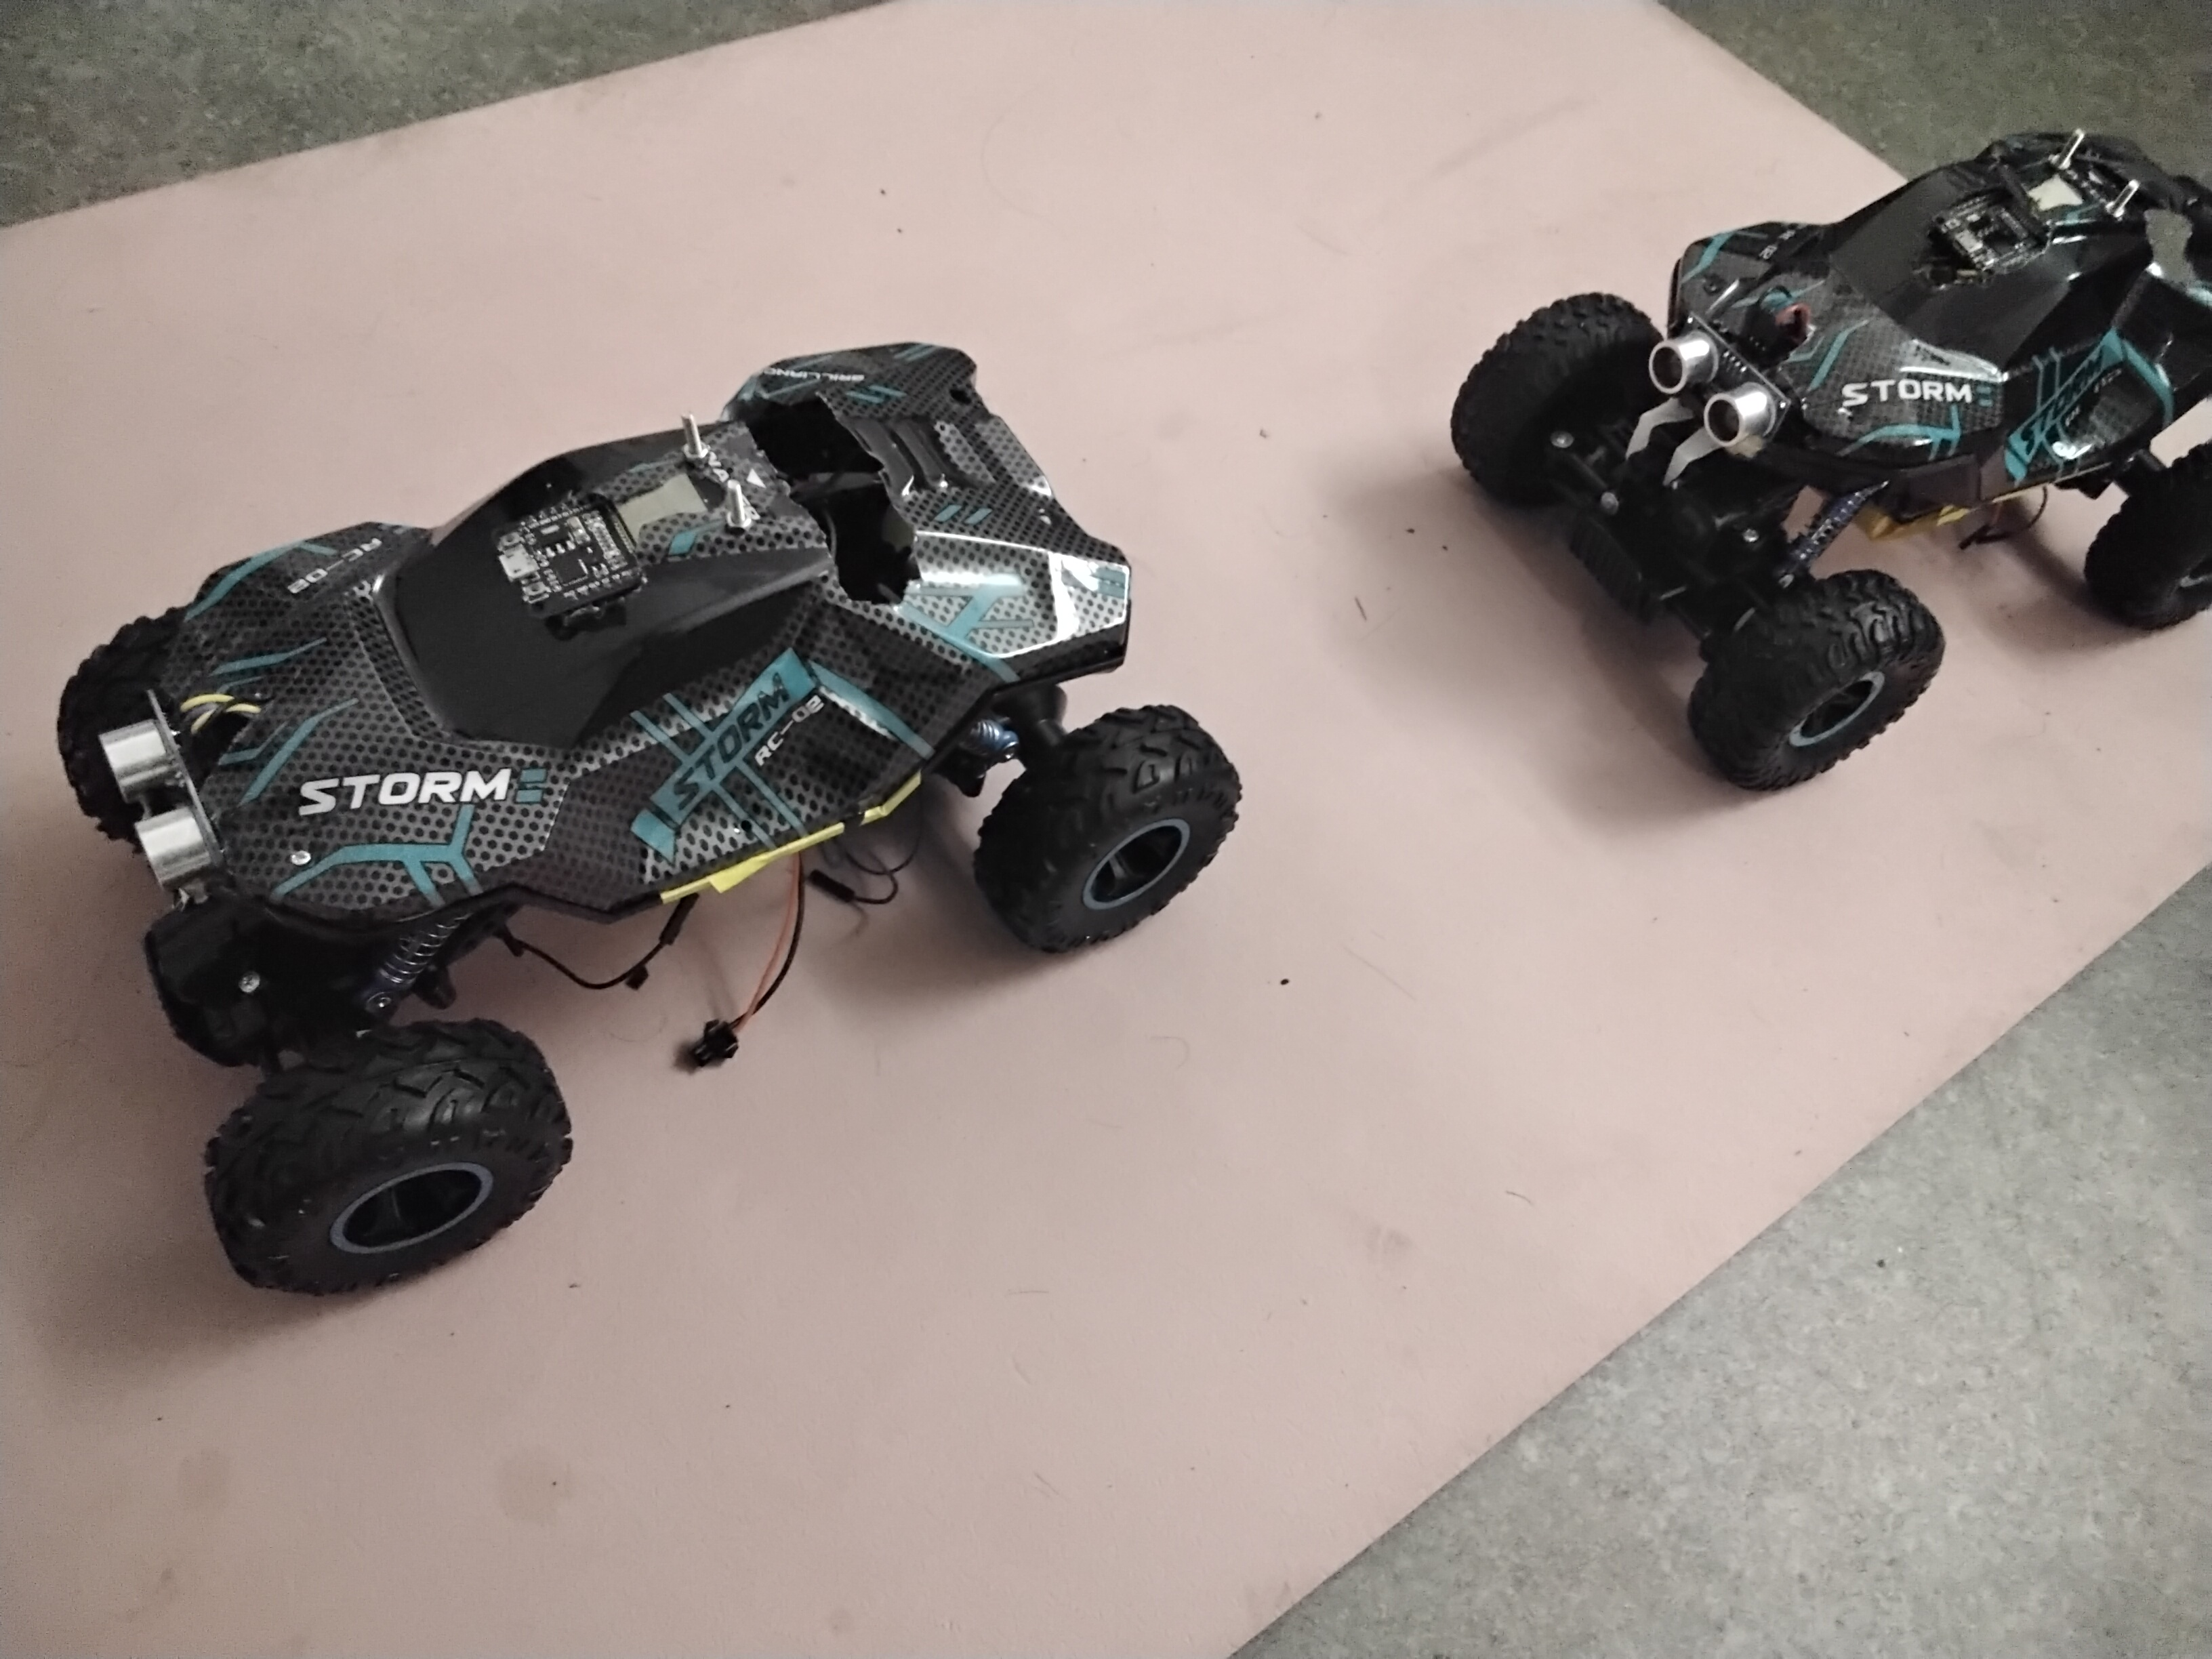
\includegraphics[width=8cm]{img/img_car.jpg}
    \caption{The experimental setup}
    \label{fig:galaxy}
\end{figure}
\section{Conclusion}
To improve the resilience of platoons using CACC against
cyberattacks on V2V communications, we propose an attack
detection and defense mechanism. By using a UIO, the state
of the preceding vehicle can be estimated without using unreliable inputs obtained through V2V communication. Simulation experiments show that the proposed detection and
defense mechanism can detect attacks with a 1-step delay and
enhance the string stability of a platoon, reducing the loss in
safety caused by attacks. It is a future work to analyze detection performances of the proposed mechanism theoretically

In this paper, we assume that there are no failures in the
on-board sensors and no delays in communication over the
network and that the controller itself is operating normally
based on the control signals. In future research, to more
closely replicate real-world situations, it will be necessary
to consider situations in which network delays occur at nondefinite times and in which the controller itself is hijacked

% In this work, a relevant problem concerning the autonomous vehicle tracking has been treated. 
% The adaptive cruise control system depends on the available measurements which need to be
% accurate as well as reliable. Firstly, a mathematical model of the vehicle was developed. 
% Secondly, the problem restriction of OMC was highlighted and its consequences on observer 
% design was pointed out. To circumvent this restriction, two methods were presented, the first 
% one consisted in discretizing the continuous-time system and shift the output in terms of time steps so a new output of the same system is generated. This output made the OMC condition 
% verified. Next, the unknown input was introduced as state variable into a discrete-time linear 
% descriptor system. After proving the detectability condition, a Lyapunov analysis of the 
% estimation error was detailed. The resulting Lyapunov equation was expressed as a Linear
% Matrix Equality (LMI) and the observer’s gain was calculated.

% \subsection{Units}
% \begin{itemize}
% \item Use either SI (MKS) or CGS as primary units. (SI units are encouraged.) English units may be used as secondary units (in parentheses). An exception would be the use of English units as identifiers in trade, such as ``3.5-inch disk drive''.
% \item Avoid combining SI and CGS units, such as current in amperes and magnetic field in oersteds. This often leads to confusion because equations do not balance dimensionally. If you must use mixed units, clearly state the units for each quantity that you use in an equation.
% \item Do not mix complete spellings and abbreviations of units: ``Wb/m\textsuperscript{2}'' or ``webers per square meter'', not ``webers/m\textsuperscript{2}''. Spell out units when they appear in text: ``. . . a few henries'', not ``. . . a few H''.
% \item Use a zero before decimal points: ``0.25'', not ``.25''. Use ``cm\textsuperscript{3}'', not ``cc''.)
% \end{itemize}

% \subsection{Equations}
% Number equations consecutively. To make your 
% equations more compact, you may use the solidus (~/~), the exp function, or 
% appropriate exponents. Italicize Roman symbols for quantities and variables, 
% but not Greek symbols. Use a long dash rather than a hyphen for a minus 
% sign. Punctuate equations with commas or periods when they are part of a 
% sentence, as in:
% \begin{equation}
% a+b=\gamma\label{eq}
% \end{equation}

% Be sure that the 
% symbols in your equation have been defined before or immediately following 
% the equation. Use ``\eqref{eq}'', not ``Eq.~\eqref{eq}'' or ``equation \eqref{eq}'', except at 
% the beginning of a sentence: ``Equation \eqref{eq} is . . .''


% \subsection{Some Common Mistakes}\label{SCM}
% \begin{itemize}
% \item The word ``data'' is plural, not singular.
% \item The subscript for the permeability of vacuum $\mu_{0}$, and other common scientific constants, is zero with subscript formatting, not a lowercase letter ``o''.
% \item In American English, commas, semicolons, periods, question and exclamation marks are located within quotation marks only when a complete thought or name is cited, such as a title or full quotation. When quotation marks are used, instead of a bold or italic typeface, to highlight a word or phrase, punctuation should appear outside of the quotation marks. A parenthetical phrase or statement at the end of a sentence is punctuated outside of the closing parenthesis (like this). (A parenthetical sentence is punctuated within the parentheses.)
% \item A graph within a graph is an ``inset'', not an ``insert''. The word alternatively is preferred to the word ``alternately'' (unless you really mean something that alternates).
% \item Do not use the word ``essentially'' to mean ``approximately'' or ``effectively''.
% \item In your paper title, if the words ``that uses'' can accurately replace the word ``using'', capitalize the ``u''; if not, keep using lower-cased.
% \item Be aware of the different meanings of the homophones ``affect'' and ``effect'', ``complement'' and ``compliment'', ``discreet'' and ``discrete'', ``principal'' and ``principle''.
% \item Do not confuse ``imply'' and ``infer''.
% \item The prefix ``non'' is not a word; it should be joined to the word it modifies, usually without a hyphen.
% \item There is no period after the ``et'' in the Latin abbreviation ``et al.''.
% \item The abbreviation ``i.e.'' means ``that is'', and the abbreviation ``e.g.'' means ``for example''.
% \end{itemize}
% An excellent style manual for science writers is \cite{b7}.


% \subsection{Figures and Tables}
% \paragraph{Positioning Figures and Tables} Place figures and tables at the top and 
% bottom of columns. Avoid placing them in the middle of columns. Large 
% figures and tables may span across both columns. Figure captions should be 
% below the figures; table heads should appear above the tables. Insert 
% figures and tables after they are cited in the text. Use the abbreviation 
% ``Fig.~\ref{fig}'', even at the beginning of a sentence.

% \begin{table}[htbp]
% \caption{Table Type Styles}
% \begin{center}
% \begin{tabular}{|c|c|c|c|}
% \hline
% \textbf{Table}&\multicolumn{3}{|c|}{\textbf{Table Column Head}} \\
% \cline{2-4} 
% \textbf{Head} & \textbf{\textit{Table column subhead}}& \textbf{\textit{Subhead}}& \textbf{\textit{Subhead}} \\
% \hline
% copy& More table copy$^{\mathrm{a}}$& &  \\
% \hline
% \multicolumn{4}{l}{$^{\mathrm{a}}$Sample of a Table footnote.}
% \end{tabular}
% \label{tab1}
% \end{center}
% \end{table}

% \begin{figure}[htbp]
% \centerline{\includegraphics{fig1.png}}
% \caption{Example of a figure caption.}
% \label{fig}
% \end{figure}

% Figure Labels: Use 8 point Times New Roman for Figure labels. Use words 
% rather than symbols or abbreviations when writing Figure axis labels to 
% avoid confusing the reader. As an example, write the quantity 
% ``Magnetization'', or ``Magnetization, M'', not just ``M''. If including 
% units in the label, present them within parentheses. Do not label axes only 
% with units. In the example, write ``Magnetization (A/m)'' or ``Magnetization 
% \{A[m(1)]\}'', not just ``A/m''. Do not label axes with a ratio of 
% quantities and units. For example, write ``Temperature (K)'', not 
% ``Temperature/K''.

% \section*{Acknowledgment}

% The preferred spelling of the word ``acknowledgment'' in America is without 
% an ``e'' after the ``g''. Avoid the stilted expression ``one of us (R. B. 
% G.) thanks $\ldots$''. Instead, try ``R. B. G. thanks$\ldots$''. Put sponsor 
% acknowledgments in the unnumbered footnote on the first page.

%\section*{References}

\begin{thebibliography}{00}
\bibitem{b1} B. Alenezi, M. Zhang, S. Hui and S. H. Żak, "Simultaneous Estimation of the State, Unknown Input, and Output Disturbance in Discrete-Time Linear Systems," in IEEE Transactions on Automatic Control, vol. 66, no. 12, pp. 6115-6122, Dec. 2021, doi: 10.1109/TAC.2021.3061993.
\bibitem{b2} J. Clerk Maxwell, A Treatise on Electricity and Magnetism, 3rd ed., vol. 2. Oxford: Clarendon, 1892, pp.68--73.
\bibitem{b3} I. S. Jacobs and C. P. Bean, ``Fine particles, thin films and exchange anisotropy,'' in Magnetism, vol. III, G. T. Rado and H. Suhl, Eds. New York: Academic, 1963, pp. 271--350.
\bibitem{b4} K. Elissa, ``Title of paper if known,'' unpublished.
\bibitem{b5} R. Nicole, ``Title of paper with only first word capitalized,'' J. Name Stand. Abbrev., in press.
\bibitem{b6} Y. Yorozu, M. Hirano, K. Oka, and Y. Tagawa, ``Electron spectroscopy studies on magneto-optical media and plastic substrate interface,'' IEEE Transl. J. Magn. Japan, vol. 2, pp. 740--741, August 1987 [Digests 9th Annual Conf. Magnetics Japan, p. 301, 1982].
\bibitem{b7} M. Young, The Technical Writer's Handbook. Mill Valley, CA: University Science, 1989.
\end{thebibliography}


\end{document}
